\chapter[ GPGPU-Based Implementation of a Finite Difference Algorithm]{GPGPU-Based Implementation of \\ a Finite Difference Algorithm}

\label{CHAPTER:CUDA}

The objective of this chapter is to give an overview of the basic implementation of an algorithm using finite difference schemes.
The source code used for the computations is based on an existing and validated version from A. Tilgner.
It was furthermore extended by the immersed boundary methods that will be explained in more detail in chapter \ref{CHAPTER:IBM}.
In this context an introduction to the aspects of GPGPU\footnote{General Purpose Computation on Graphics Processing Uni}-Computing
with the CUDA \footnote{Computing Uniform Device Architecture} architecture will be given.
For the computations in this thesis Tesla C1060 and Tesla K20m GPUs by NVIDIA were used. %, the complete system configurations can be looked up at (AX.X).
In this chapter all informations related to GPGPU-Computing and CUDA are adapted from the CUDA Programming Guide and the CUDA Best Practices Guide from NVIDIA
\citep{CUDAPG}, \citep{CUDABP}. All details about the implementation of the algorithm were obtained by studying the source code
and from private communication with A.Tilgner.

\section{GPGPU-Computing with CUDA}

CUDA is an architecture developed by NVIDIA to enable an easy approach to the implementation of GPGPU-based algorithms.
The underlying idea is to hide the complexity of the hardware under a more high oriented and generalized software abstraction layer.
This is done by introducing some additional programming language extensions for example in C/C++.
Furthermore it is necessary to use a CUDA suited compiler like NVCC.

\subsection{Hardware and Memory Architecture}

A cuda device contains an array of so called streaming multiprocessors (SM).
Each of these SMs contains a group of small execution units, which are called cuda cores.
For the exchange of data between different SMs, cuda cores and the CPU side of the computer, there exist different
types of memory, as shown  in Fig.  \ref{fig:gpu_memory_layout}.
\newpage

\begin{figure}[!tbp]
      \centering
        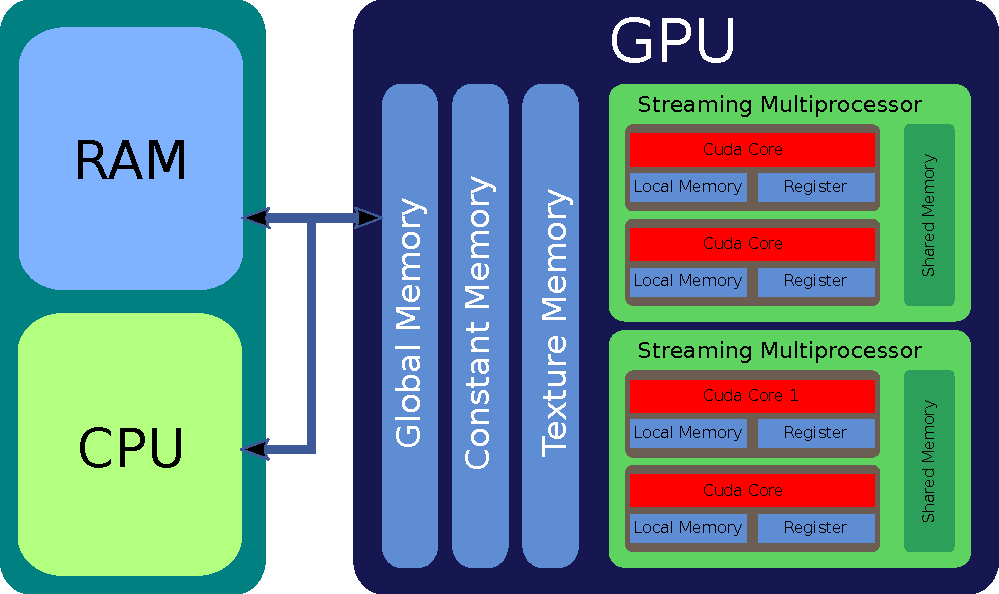
\includegraphics[width=0.9\textwidth]{gfx/cuda/gpu.pdf}
          \caption{Memory layout of a Nvidia-GPU}
    \label{fig:gpu_memory_layout}
\end{figure}

\begin{description}
    \item[Global Memory] The global memory is the largest memory on the GPU and can be accessed by all cuda cores.
                         It is  used to exchange data with the RAM and distribute it between different SMs.
                         Writing and reading from the global memory is slow. A part of the global memory can furthermore be used as a constant memory.
                         In this case multiple memory accesses on the same location are temporary cached.
                         In addition the use of the global memory as a texture memory is possible. The memory access is then spatially cached.


    \item[Shared Memory] Each SM contains a shared memory, much smaller than the global memory \footnote{Around 16kb on c1060 and 64kb on k20m}. It is accessible
                         by all cuda cores of the SM.
                         This memory type is much faster (x100) than the global memory and is usefull when multiple operations
                         by different cuda cores of one SM are carried out on the same data.

    \item[Register / Local Memory] Each cuda core possesses an own set of registers and local memory.
                                   The register access is slightly faster than the access  on the shared memory.
                                   Local memory access is very slow since the storage is
                                    created on the global memory, when a cuda core runs out of registers.
\end{description}

\clearpage

\subsection{Thread Management}
\label{cuda:sec_threadmanage}

In order to distribute the workload between different SMs and cuda cores an additional syntax is necessary.
The CUDA API therefore  introduces the notion of a thread and a block.

\begin{description}
    \item[Thread] A Thread is the software abstraction of a single cuda core. It can be identified with
                   a maximum of three IDs, \textbf{threadIdx.x}, \textbf{threadIdx.y} and\textbf{threadIdx.z}.

    \item[Block] A block is defined as a group of threads, i.e. in Fig. \ref{cuda:grid_example} a block contains 64 threads.
                 There  is no direct hardware equivalent to a block.
                 A block is identified by a maximum of two IDs, \textbf{blockIdx.x} and \textbf{blockIdx.y}

    \item[Blocksize] The blocksize is defined before running a function on the GPU. It determines how
                    many threads run inside a block. In Fig. \ref{cuda:grid_example} the blocksize is set to (8, 8) and
                    each thread is defined by a \textbf{threadIdx.x} and \textbf{threadIdx.y}.

    \item[Gridsize] The gridsize defines the total number of blocks, i.e. (2, 2) in the example.
\end{description}

The concept of a grid containing blocks of threads is a little bit confusing at first.
However these abstractions are necessary to enable a high and parallelized workload on the GPU,
since each block can be dynamically assigned to a different SM.


\begin{figure}[!bp]
      \centering
        \resizebox{0.5 \textwidth}{!}{
       \import{gfx/cuda//}{grid.pdf_tex}
        }
       \caption{Thread management of the CUDA API, exeplarily shown for a
        grid of blocks.  Each block contains a sub-grid with 8x8 threads.}
       \label{cuda:grid_example}
\end{figure}


\subsection{Performance Considerations}

For the programming of a CUDA device a vast number of optimization techniques exist (see \citep{CUDABP}),
to explain all of these methods would go beyond the scope of this thesis.
Here a short description of the most import ones is given

\begin{description}
    \item[Memory Coalescing]
        During the runtime a SM executes a number of 32 threads in parallel, this thread group is denoted as a warp.
        In order to enable a fast memory access on the global memory, threads which are adjacent in a warp should read from adjacent memory cells.
        This access pattern is denoted as coalesced memory access. Inhomogeneous access pattern on the global memory can lead to so called bank
        conflicts, as a result the performance of a cuda program can drastically decrease.

    \item[Sparse global memory access]
        The global memory should be used for data transfer and distribution with as little as possible global reads and writes.
        This reason for this approach is the slow global memory access ($\times 100$) in comparison to a fast shared memory access.

    \item[Branch Divergence] All threads in a single branch should execute the same command.
                              Conditional statements like \texttt{if..then..else} create divergent code.
                              The execution is performed serial and the performance decreases.
\end{description}


\subsection{Simulation Domain and  Memory Layout}

The three-dimensional simulation domain is given by a cuboid that is discretized by a
collocated cartesian grid with a constant step size in each direction.
From here on the following conventions will be used.

\begin{description}
    \item[$l_i$] The length of the cuboid in $x$, $y$ or $z$ direction, $i\in{x, y, z}$
    \item[$N_i$] The number of grid points in $x$, $y$ or $z$ direction, $i\in{x, y, z}$
    \item[$\Delta i$] The step size between to grid points in $x$, $y$ or $z$ direction, $i\in{x, y, z}$
\end{description}

A single grid point is determined by the set of indices $i,j,k$ where ${0\leq i < N_x}$,
${0\leq j < N_y}$ and ${0\leq k < N_z}$. The position vector is given by ${\vec{r} = (i\cdot\Delta x, j\cdot \Delta y, k\cdot \Delta z)^T}$.
Each grid point lies in the center of a grid cell of size $\Delta x \cdot \Delta y \cdot \Delta z$,
since a collocated grid is used all variables are located in the cell center.
\footnote{For example on a staggered grid, the velocity components are stored on the cell faces.}
For the computation a variable $\Phi\in\{v_x, v_y, v_z, \rho\}$, is stored into three registers

\begin{description}
    \item[$C_\Phi$] Located on the RAM. Used mainly for data transfer and analysis
    \item[$R_\Phi$] Located on the global memory on GPU. A variables is stored here after the computation of a time step.
    \item[$B_\Phi$] Located on the global memory on GPU. This is the buffer register for the Williamson RK scheme, see Sec. \ref{numerik:rk_williamson_sec}.
\end{description}

The size of a storage register is given by $(N_x+4)(N_y+4)(N_z+4)$.
An additional offset $+4$ is given since two additional layers of ghost points are attached to each side of the simulation domain.
This points are used for a computation of the boundary conditions, see Sec. \ref{sec:cuda_boundaries}.
All registers have a one dimensional memory layout.
Hence, the register position of a grid point is calculated by

\begin{align}
    P(i, j, k) = i(N_y+4)(N_z+4)+j(N_z+4)+k
\end{align}

which is a row-major access pattern.

\section{Time Step Algorithm}
\label{sec:cuda_timestep}

In this section an overview of the computation of a single time step will be given.
For this example the Navier-Stokes equation, given by Eq. \ref{theorie:eqns}, will be used.
Before the computation of the time step all initial conditions are saved to the
registers $C_{\Phi}$ and  $R_{\Phi}$.
The time integration is performed with the Willamson-RK3 scheme, see Sec. \ref{numerik:rk_williamson_sec}.
This schemes consist of three sub time step, in this example only the first step given by

\begin{align}
    \begin{split}
    Q_1 = \Delta t \mathcal{L}^*\left(\Phi^n\right)\qquad &\Rightarrow \qquad \Phi^{1} = \Phi^n + \frac{1}{3}Q_1
    \end{split}
\end{align}

will be considered.  The computation of the remaining steps is similar.


The simulation domain is divided into a grid of  $N_y/8 \times N_z/8$ blocks. On each of these blocks the integration is performed separately.
This segmentation is similar to the example introduced in Sec. \ref{cuda:sec_threadmanage} (see Fig. \ref{cuda:grid_example}), except an
additional index \textbf{threadIdx.z} is used.
This index seperates the variables during the integration
\footnote{For example, for $\rho$ it is threadIdx.z = 0, for $v_x$  it is threadIdx.z=1 and so forth.},
with this convention each block contains a total number of 8x8x4 threads.

For a computation of the finite difference schemes  a 5-Point stencil is used, as shown in Fig. \ref{cuda:stencil}.
Each cell in this Stencil corresponds to one grid cell in the numerical domain.
The inner points of the stencil are enumerated with 1, the outer with 2. For example in $x$ direction the points are denoted as West2,
West, Center, East and East2 in $x$ direction or with the abbreviations W2, W1, C, E1 and E2.
For second order finite difference schemes, only the inner points  are used, we refer to a 3-Point stencil in this case.

\begin{figure}[!bp]
      \centering
        \resizebox{0.6\textwidth}{!}{
       \import{gfx/cuda//}{stencil.pdf_tex}
        }
        \caption{
            5-Point stencil used for the discretization, with the directions North, West, South, East, Up, Down and th Center.
        }
       \label{cuda:stencil}
\end{figure}

\begin{figure}[!bp]
      \centering
        \resizebox{0.6\textwidth}{!}{
       \import{gfx/cuda//}{timestep.pdf_tex}
        }
       \caption{
           Shared memory block location in the simulation domain during a time step. With the center points (C), additional loaded boundary  points (B)
           and the next layer (NL).
       }
       \label{cuda:timestep_algo_img}
\end{figure}
\clearpage

The computation of one time step can be separated into an initialization part and a for-loop which iterates by the index $i$, over the simulation domain.
In the initialization part a block from the simulation domain is loaded into the shared memory of the GPU.
As a first step each thread is assigned to a grid point $(i, j, k)$.

\begin{align}
    \begin{split}
    i &= 2\\
    j &= \text{blockIdx.x}\cdot 8 + \text{threadIdx.y} + 2\\
    k &= \text{blockIdx.y}\cdot 8 + \text{threadIdx.x} + 2
    \end{split}
\end{align}

%The offset 2 is a again result of the ghost points, more on this in Sect. ()
The position of the center $C$ for each thread, is then given by $P(i, j, k)$.
Then each thread has to load the neighbor points W2, W1, E1 and E2.
The offset to $C$ is given by a multiple of ${L=(N_y+4)(N_z+4)}$, for example ${W2= C - 2L}$.
Furthermore, on the sides of the Block additional boundary points (B) are necessary for the discretization
in the directions U, D, N and S.
With the calculated positions the variables are now loaded into the shared memory of the GPU.
Fig. \ref{cuda:timestep_algo_img} shows how this memory structure is located in the simulation domain  for $i>2$.
The 5-Point stencil is exemplarily shown for one center point and the boundary points (B) on the sides of the block are shown.
The initialization procedure is now finished.

In the first step of the for-loop the spatial derivatives are computed.
Since these terms are quite large this will be shown exemplarily for the laplace operator,
with a central difference scheme of fourth order, given by Eq. \ref{num:fd_o4_methods}, for the $v_x$ component.

\begin{align}
    \begin{split}
    \Delta v_x   \approx &  \frac{1}{12\Delta x^2} \left(-v_x(i+2, j, k) + 16v_x(i+1, j, k) - 30v_x(i, j, k) + 16v_x(i-1, j, k)-v_x(i-2, j, k)\right)\\
                              +&  \frac{1}{12\Delta y^2} \left(-v_x(i, j+2, k) + 16v_x(i, j+1, k) - 30v_x(i, j, k) + 16v_x(i, j-1, k)-v_x(i, j-2, k)\right)\\
                              +&  \frac{1}{12\Delta z^2} \left(-v_x(i, j, k+2) + 16v_x(i, j, k+1) - 30v_x(i, j, k) + 16v_x(i, j, k-1)-v_x(i, j, k-2\right))
    \end{split}
\end{align}

The intermediate step $Q_{\Phi}$ is than computed with the conditionals
\begin{center}
 \begin{minipage}{.55\linewidth}
\begin{algorithmic}
\IF {(threadIdx.z==0)}
      \STATE ${Q_{\rho} = -\nabla \vec{v}}$
\ENDIF
\IF {(threadIdx.z==1)}
      \STATE ${Q_{v_x} = -(\vec{v} \nabla) v_x - c^2\partial_x\rho + \frac{1}{\Rey}\partial^2_xv_x + f_x}$
\ENDIF
\end{algorithmic}
 \end{minipage}

\clearpage

 \begin{minipage}{.55\linewidth}
\begin{algorithmic}
\IF {(threadIdx.z==2)}
      \STATE ${Q_{v_y} = -(\vec{v} \nabla) v_y - c^2\partial_y\rho + \frac{1}{\Rey}\partial^2_yv_y + f_y}$
\ENDIF
\IF {(threadIdx.z==3)}
      \STATE ${Q_{v_z} = -(\vec{v} \nabla) v_z - c^2\partial_z\rho + \frac{1}{\Rey}\partial^2_zv_z + f_z}$
\ENDIF
\end{algorithmic}
 \end{minipage}
\end{center}

where $(f_x, f_y, f_z)^T = \vec{F}_{\text{ext.}}$. The advection term $(\vec{v}\nabla)\vec{v}$ is discretized by the third-order upwinding scheme from Sec. \ref{num:sec_para:upwindingscheme}
and all remaining derivatives are approximated with the fourth order finite difference schemes from Eq. \ref{num:fd_o4_methods}.
An alternative lower order implementation uses the second order finite difference methods.
After this step the computation for the center points (C) is finished.
The results are stored in the buffer registers $R_\Phi$.

In the next pass of the loop the index $i$ is incremented and the algorithm loads the next layer (NL) as indicated in Fig.\ref{cuda:timestep_algo_img}.
All other layers are shifted by one position, With this approach each layer only gets loaded once in the shared memory.
After the for-loop has iterated over the simulation domain the first part of the time step is finished.
The remaining computation is
\begin{align}
     \Phi^{1} = \Phi^n + \frac{1}{3}Q_1
\end{align}

The algorithm for this computation performs identical except no derivatives need to be calculated, and
the border points (B) are redundant.

\subsection{Boundary Conditions}
\label{sec:cuda_boundaries}

For the implementation of the boundary conditions two additional layer of grid points are added on each side of the simulation domain.
In this section the implementation of boundary conditions is presented for the one-dimensional case in $x$-direction.

\paragraph{No-Slip Boundaries}\mbox{}\\

Consider the left side of the simulation domain.
The ghost points are given by the points ${g_{l2}=(0, j, k)}$, ${g_{l1}=(1, j, k)}$,
the boundarie is at ${b=(2, j, k)}$ where $\vec{v}=0$ and the next inner points are
$i_{l1}=(3, j, k)$ and $i_{l2}=(4, j, k)$.
For No-Slip boundaries the velocity profile is mirrored and inverted at $b$.
\begin{align}
    v_x(g_{l2}) = -v(i_{l2}) \qquad ; \qquad v(g_{l1}) = -v(i_{l1})
\end{align}
The same procedure is performed for $v_y$ and $v_z$.
Due to the symmetry of the velocity profile on the boundary the viscous stress vanishes and $\partial_t\vec{v} = 0$. Hence, $\vec{v}(t)=0$.


\paragraph{No-Flux Boundaries}\mbox{}\\

Consider the left side of the simulation domain.
The ghost point are given by the points ${g_{l2}=(0, j, k)}$, ${g_{l1}=(1, j, k)}$,
the boundary is set to  ${b=(2, j, k)}$ and the next inner points are
$i_{l1}=(3, j, k)$ and $i_{l2}=(4, j, k)$.
For No-Flux boundaries it is necessary that $\partial_x\Phi = 0$ for any variable $\Phi$.
By setting

\begin{align}
    \Phi(g_{l2}) = \Phi(i_{l2})\qquad ; \qquad \Phi(g_{l2}) = \Phi(i_{l1})
\end{align}
it follows that
\begin{align}
    \pdn[\Phi]{x} = \frac{1}{12\Delta x}{-\Phi(g_{l2})+8\Phi(g_{l1}) -8\Phi(i_{l1}) + \Phi(i_{l2})} = 0
\end{align}

with the use of a fourth order central difference scheme.
This boundary condition is used for $\rho$ to satisfy the mass conservation.

\paragraph{Free-Slip Boundaries}\mbox{}\\

The Free-Slip boundaries are implemented by using No-Flux boundaries for
the $v_y$ and $v_z$ components and No-Slip boundaries for the $v_x$ component.

\paragraph{Periodic Boundaries}\mbox{}\\

Consider the ghost points $g_l2=(0, j, k)$, $g_l1=(1, j, k)$ and the inner points $i_{l1}=(2, j, k)$ and $i_{l2}=(3, j, k)$ on the left side of
the simulation domain.
On the right sides of the simulation domain the ghost points are $g_r2=(N_x+1, j, k)$, $g_r1=(N_x, j, k)$
and the inner points $i_{r1}=(N_x-1, j, k)$ and $i_{r2}=(N_x - 2, j, k)$.
For periodic boundaries the regions on the left and right side of the simulation domain are simply exchanged by

\begin{align}
    v_x(g_{l2}) = v(i_{r2}) \qquad ; \qquad v(g_{l1}) = v(i_{r1})\\
    v_x(g_{r2}) = v(i_{l2}) \qquad ; \qquad v(g_{r1}) = v(i_{l1})
\end{align}


%\subsection{Remarks}
%-performance blabla
%-tilgner bsp
%-threads
%
%- measurements / output
%- zusammenfassung flow diagramm
%- erläuterung threads
%- python api
%
%-performance blabla
%-tilgner bsp
%-threads
%- measurements / output
%- zusammenfassung flow diagramm
%- erläuterung threads
%- python api

%During execution time each cuda core is executed as a thread, in an SIMD\footnote{Single Instruction Multiple Device}-like behaviour.
%This means every cuda core on one SM executes the same instruction set simultaneously. To differentiate between different cuda cores,
%each get assigned to a different \textbf{ThreadId}.
%With the declaration of a block dimension, we define how many threads are executed in parallel.
%The block dimension can be up to 3-dimensions. In this case each cuda core will be assigned to a ThreadId in x, y and z direction.
%A collection of threads with this grid structure is called a block.
%Since the


